\documentclass{beamer}

\usepackage{fontspec}
\usepackage{xeCJK}
\setCJKmainfont{DFFN_R3.TTC}
\XeTeXlinebreaklocale "zh"
\XeTeXlinebreakskip = 0pt plus 1pt
\linespread{1.3}
\allowdisplaybreaks

\newcommand{\weib}{\CJKfamily{weib}}
\newcommand{\hkss}{\CJKfamily{hkss}}
\newcommand{\hksy}{\CJKfamily{hksy}}
\newcommand{\lth}{\CJKfamily{lth}}
\usepackage{color}
\usepackage{booktabs}
\usepackage{tabularx}
\usepackage{caption}
\usepackage{tikz}
\usepackage{verbatim}
\usepackage{pgfplotstable}
\pgfplotsset{width=12cm}
\pgfplotsset{height=7cm}
\pgfplotsset{compat=1.13}

\usetheme{EastLansing}
\usetikzlibrary{positioning}
\useinnertheme{rectangles}
\usefonttheme{professionalfonts}

\newcommand{\lw}{0.8mm}
\setbeamercovered{transparent}


%\AtBeginSection[]
%{
  %\begin{frame}<beamer>
	%\frametitle{報告大綱}
	%%\frametitle{RoadMap}
    %\tableofcontents[currentsection]
  %\end{frame}
%}

\title{CS Seminar Report}
\subtitle{\textcolor[rgb]{0.00,0.50,1.00}{{Adversarial Attack/Defense in Machine Learning}}}
\author{徐瑞陽}
\date{2019/04/29}
\begin{document}



\begin{frame}
\maketitle
\end{frame}

\begin{frame}
\frametitle{Outline}
\tableofcontents
\end{frame}

\section{Motivation}
\begin{frame}{Motivation}
  \begin{itemize}
    \item We want to deploy ML classifiers in \textbf{real world}.
    \item The classifiers that are robust to noises in nature and work ``most of the time'' is not sufficient
    \item We want our model robust to the inputs built specifically to fool it
  \end{itemize}
\end{frame}

\begin{frame}{ML Model Are Accurate but Brittle}
  \footnote{source: \href{http://metalearning-symposium.ml/files/vinyals.pdf}{Explaining and Harnessing Adversarial Examples, ICLR 2015}}
  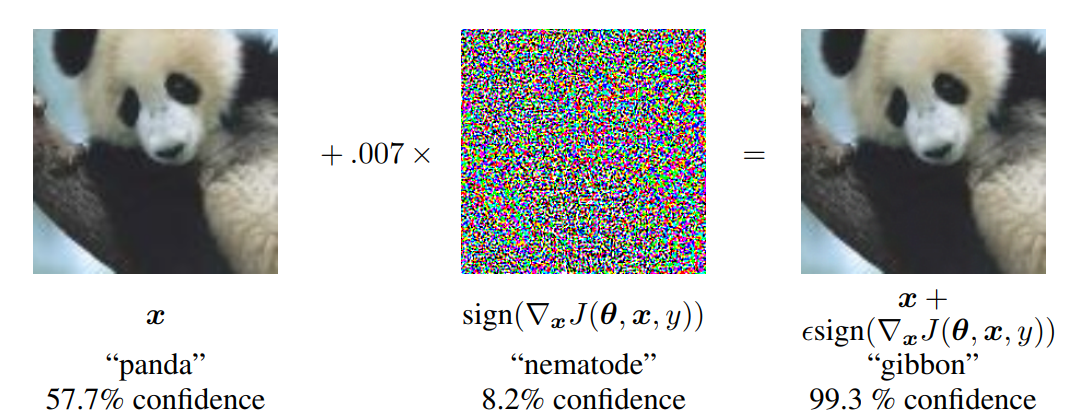
\includegraphics[width=\textwidth]{fig/idea.png}
\end{frame}

\section{Definition}
\begin{frame}{Optimization View on Adversarial Robustness}
  \begin{block}{Objective}
    \[ \min_\theta \mathbb{E}_{(x,y) \sim \mathcal{D}}[\max_{\delta \sim \mathcal{S}}L(x+\delta,y|\theta)]\]
  \end{block}
  \begin{itemize}
    \item $\mathcal{S}$: allowed pertubations of adversary
    \item $\theta$: weights of classifier model
    \item $\mathcal{D}$: data distribution
  \end{itemize}
\end{frame}


\begin{frame}{Allowed Pertubations of Adversary}
  \begin{block}{Want}
    $\delta$ is small (which depends on the application)
  \end{block}
  \begin{itemize}
    \item $L_p$ norm $\leq \epsilon$
      \begin{itemize}
        \item $L_0$: \# of pixel can change
        \item $L_2$: move within Euclidean ball with radius $\epsilon$
        \item $L_\infty$: every pixel has $\epsilon$ budget to move around
      \end{itemize}
    \item Rotation or translation
  \end{itemize}
\end{frame}

\begin{frame}{Amount of Information Adversary Had}
    \begin{itemize}
      \item White-Box: Adversary has \textbf{full-access} to the model (structure, weight)
      \item Black-Box: Labels assigned by the \textbf{Oracle} for chosen input (e.g API call)
    \end{itemize}
\end{frame}

\begin{frame}{Optimization Methods of Adversary}
  How to find the most adversarial point within $\mathcal{S}$?
  \begin{itemize}
    \item Gradient (First Order Adversary), the most common one
    \item Mixed Integer Programming \\
      $\rightarrow$ \href{https://openreview.net/forum?id=HyGIdiRqtm}{Evaluating Robustness of Neural Networks with Mixed Integer Programming, ICLR2019}
      
    \item And more...
  \end{itemize}
\end{frame}

\begin{frame}{One Adversary Instance - FGSM}
  \textit{Fast Gradient Sign Method \footnote{source: \href{http://metalearning-symposium.ml/files/vinyals.pdf}{Explaining and Harnessing Adversarial Examples, ICLR 2015}}} is an \color{blue}{$L_\infty\text{-bounded}$}  \color{purple}{first-order} \color{orange}{white-box} \color{black}{adversary}
  
  \[
    \tilde{x} = x + \epsilon \, \texttt{sgn} \nabla_xL(x,y|\theta)
  \]

  Some variants as follows
  \begin{itemize}
    \item multi-step (possibly w/ projection)
    \item ensemble
    \item proxy model $\theta^\prime$ (black-box setting)
  \end{itemize}
\end{frame}

\section{Trade-off Between Standard Accuracy \& Adversarial Robustness}

\begin{frame}
    \center \LARGE{Why not just train with all adversarial samples?}
\end{frame}

\begin{frame}
    \center \LARGE{Is adversarial robustness FREE?}
\end{frame}

\begin{frame}{Trade-off of Adversarial Robustness}
  \begin{itemize}
    \item More training time
    \item \textbf{Generalization accuracy drops} \footnote{source: \href{http://metalearning-symposium.ml/files/vinyals.pdf}{Robustness May be at Odds with Accuracy, ICLR 2019}}
  \end{itemize}
\end{frame}

\begin{frame}{Example: Binary Classification Task}
  Consider binary classification task, $(x,y) \sim \mathcal{D}$ as follows
  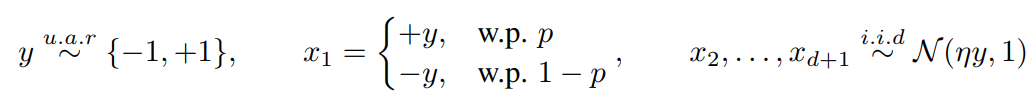
\includegraphics[width=\textwidth]{fig/cls.png}
  We choose $\eta$ be large enough to separate these 2 distributions ($\eta = \Theta(1/\sqrt{d})$)  

  \begin{itemize}
    \item $x_1$ is \textit{moderately correlated} with the label
    \item $x_2 \sim x_{d+1}$ is \textit{very weakly correlated} with the label
  \end{itemize}
\end{frame}

\begin{frame}{Standard Classification is Easy}
  \begin{block}{Observation}
    Although each $x_2 \sim x_{d+1}$ feature is weakly correlated, the average of them is \textit{highly correlated} 
  \end{block}
  Consider a linear classifier $f_{avg}$

  \[
    f_{avg}(x) := \texttt{sgn}(w_{unif}^T x), \quad \text{where} \, w_{unif}:= \Big[0,\frac{1}{d},\cdots,\frac{1}{d}\Big]
  \]

\end{frame}

\begin{frame}{Standard Classification is Easy (cont.)}
  \begin{block}{Linear classifier}
  \[
    f_{avg}(x) := \texttt{sgn}(w_{unif}^T x), \quad \text{where} \, w_{unif}:= \Big[0,\frac{1}{d},\cdots,\frac{1}{d}\Big]
  \]
  \end{block}
  Standard accuracy is 
    \begin{align*}
      \Pr[f_{avg}(x) = y] &= \Pr[\texttt{sgn}(w_{unif}^T x) = y]  \\
                          &= \Pr \Big[\frac{y}{d}\sum_{i=1}^d \mathcal{N}(\eta y,1) > 0 \Big] \\
                          &= \Pr \Big[\mathcal{N}(\eta,\frac{1}{d}) > 0 \Big]
    \end{align*}

  which is $> 99\%$ when $\eta \geq 3 / \sqrt{d}$
\end{frame}

\begin{frame}{Adversarially Robust Classification}
  Consider moderate pertubation $\delta$, which $L_p \leq \epsilon = 2 \eta$...\\
  Those correlated features become \textbf{anti-correlated}

  Adversarial accuracy is
    \begin{align*}
      \Pr[\texttt{sgn}(x + \delta) = y] &= \Pr \Big[\frac{y}{d}\sum_{i=1}^d \mathcal{N}(-\eta y,1) > 0 \Big] \\
                                &= \Pr \Big[\mathcal{N}(-\eta,\frac{1}{d}) > 0 \Big]
    \end{align*}

  The classifier derived before cannot get adversarial accuracy better than $1\%$
\end{frame}

\begin{frame}{Some Lessons}
  \begin{itemize}
    \item For standard classifier, any feature which is weakly correlated is useful, so the model will exploit them
    \item On the other hand, adversary can also simply exploit these features by a moderate $\epsilon$ (where $\epsilon = \mathcal{O}(1/\sqrt{d})$)
  \end{itemize}
\end{frame}

\begin{frame}{Theorem: Robustness-accuracy trade-off}
  Any classifier that attains at least $1 - \delta$ standard accuracy on $\mathcal{D}$ has robust accuracy at most $\frac{p}{1-p}\delta$ against $L_\infty$-bounded adversary with $\epsilon \geq 2 \eta$
\end{frame}

\begin{frame}{Discussion of robust/non-robust features}
  In above case
  \begin{itemize}
    \item $x_1$: robust feature (something invariant)
    \item $x_2 \sim x_{d+1}$: non-robust feature
  \end{itemize}
  \begin{block}{Claim}
    Standard classifier assigns weight to even weakly correlated features, \\but robust classifier doesn't assign any weight beyond a certain threshold
  \end{block}
\end{frame}

\begin{frame}{Experiments: Binary Linear classifier on MNIST (5 vs 7)}
  \center{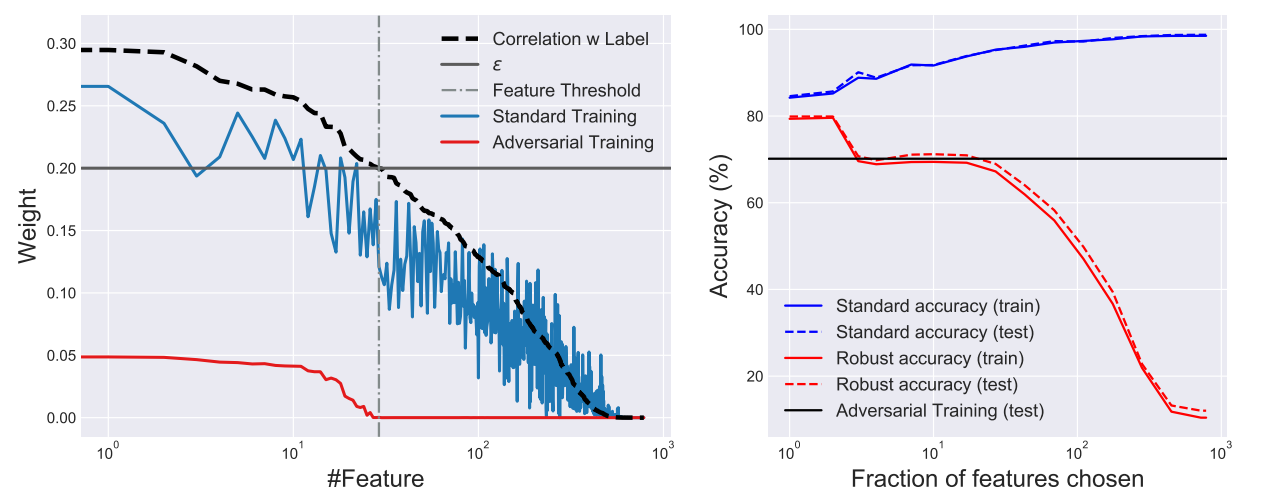
\includegraphics[width=0.8\textwidth]{fig/p2/cu.png}}\\
  Right figure: \\Both accuracy is trained using \textbf{standard} training with subset of features \\
(w/ decreasing relation between label, calculated thru $\mathbb{E}_{(x,y) \sim \mathcal{D}}[yx_i]$)
\end{frame}


\begin{frame}{Experiments: Multi-class classification}
  \center{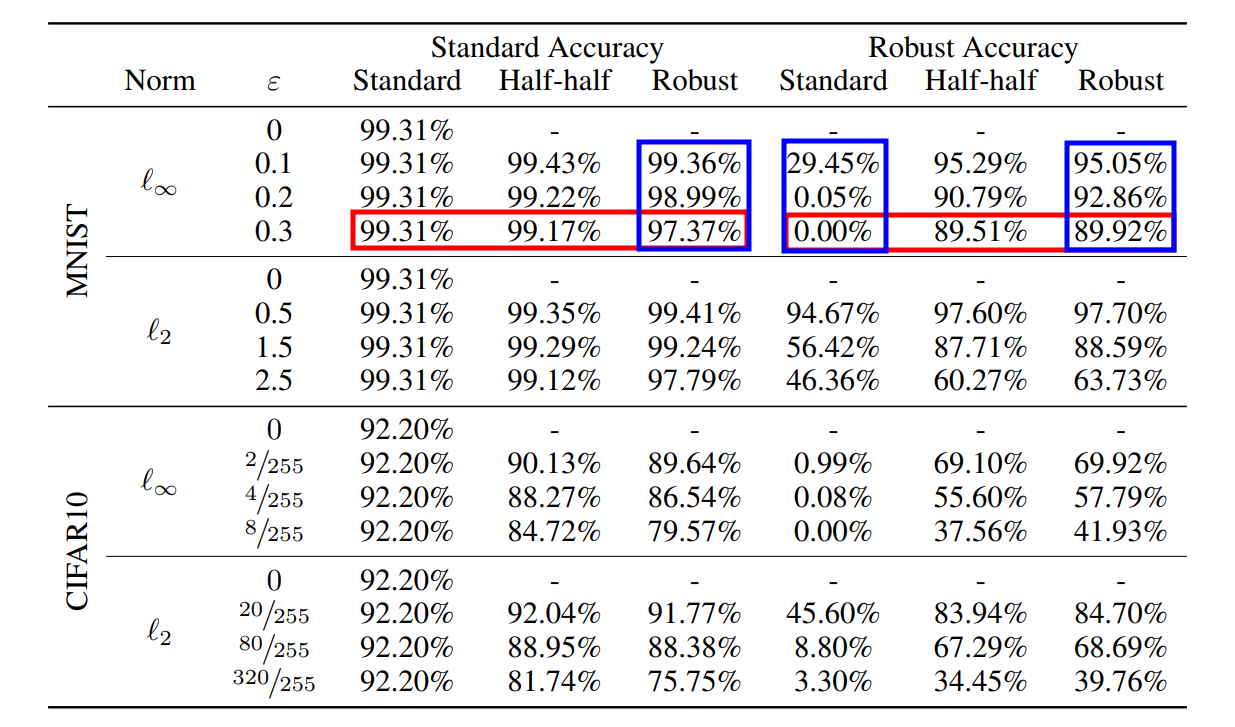
\includegraphics[width=\textwidth]{fig/exp.png}}\\
\end{frame}

\section{Other Interesting Aspects}
\begin{frame}{Other Interesting Aspects}
  \begin{itemize}
    \item Transferability of adversarial examples
      \begin{itemize}
        \item Intra-technique: That's why black box attack still works well
        \item Cross-technique: e.g Decision Tree vs NN (even one is differentiable model, one is not)
      \end{itemize}
    \item Obfuscated gradients: Over-confidence of adversarial robustness (ICML2018)
  \end{itemize}
\end{frame}

\begin{frame}
  \begin{center}
    \weib{\LARGE{謝謝聆聽!}}
    %\LARGE{Questions?}
  \end{center}
\end{frame}




%\begin{frame}{Interpretable gradients}
  %Loss gradients in the input space align well with human eyes
  %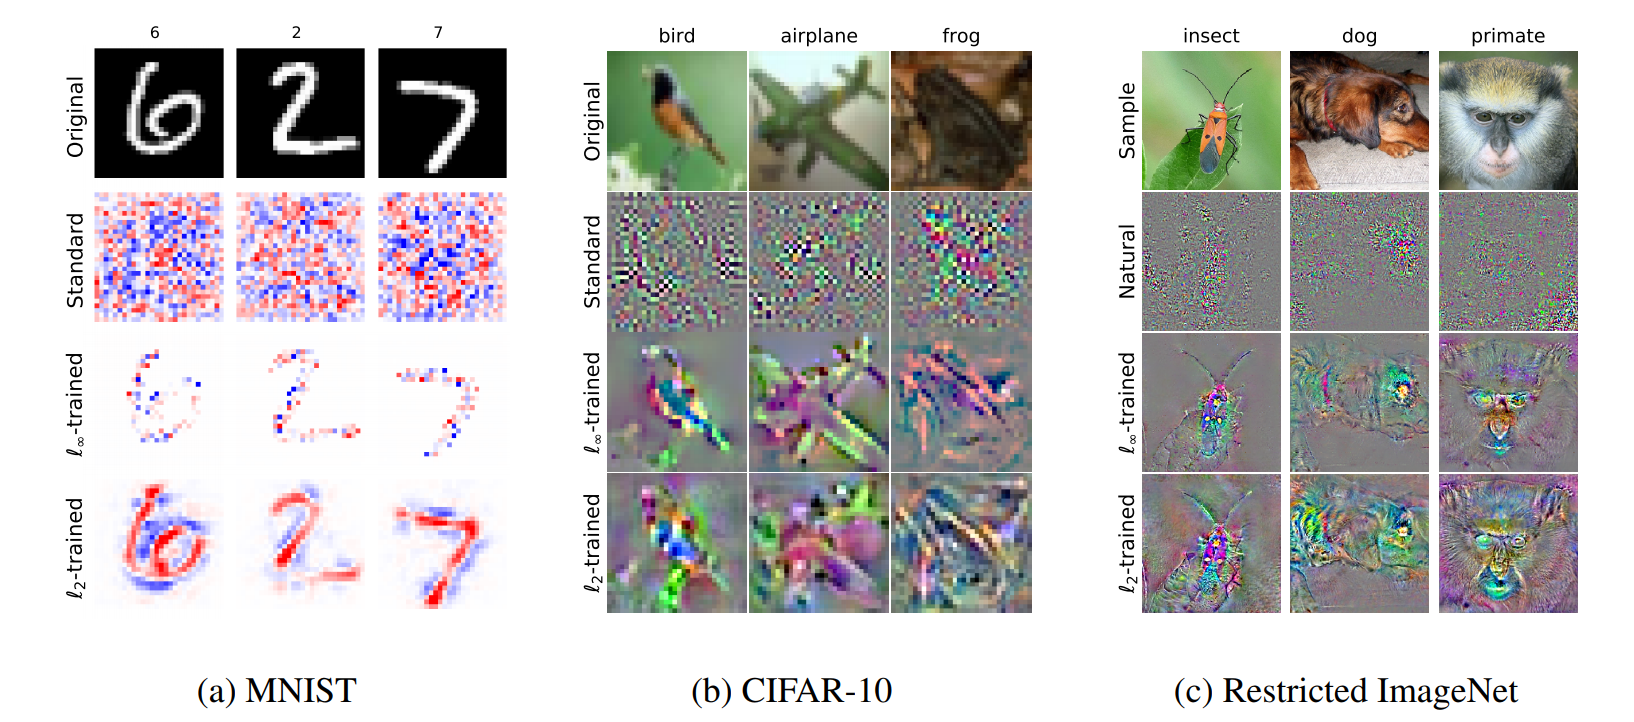
\includegraphics[width=\textwidth]{fig/p2/int-grad.png}
%\end{frame}

%\begin{frame}{Some Thoughts}
  %\begin{itemize}
    %\item By encoding appropriate prior into set of pertubations $\mathcal{S}$, adversarial training can provide interpretable gradients 
  %\end{itemize}
%\end{frame}

\end{document} 
